\documentclass{article}
\usepackage{graphicx}

\date{\today}
\author{Tarik Atlaoui \\ Nicolas Peugnet \\ Kimmeng Ly \\ Max Eliet}

\begin{document}


\begin{titlepage}
	\enlargethispage{2cm}
	\newcommand{\HRule}{\rule{\linewidth}{0.5mm}}
	\center
	\textsc{\LARGE
	Pre-rapport du PSAR 
	} \\[1cm]
	\HRule \\[0.4cm]
	{ \huge \bfseries API générique pour le développement d'applications réparties \\[0.15cm] }
	\HRule \\[4cm]
	\large{Tarik Atlaoui \\[3mm] Nicolas Peugnet \\[3mm] Kimmeng Ly \\[3mm] Max Eliet} \\[3cm]
	09 Mars 2020 \\[3cm]
%	\hfill 
\includegraphics[width=5cm]{logoSU.jpg}
\end{titlepage}

	\newpage
	\pagenumbering{arabic}
		\section{Introduction}
			\large{
			\indent Notre projet a pour but d'implémenter un intergiciel permettant l'execution d'applications réparties, aussi bien sur une infrastructure réelle que sur un simulateur, sans avoir à en modifier le code, afin de simplifier le développement de futures applications réparties.
\\[2mm]
			 \indent Dans notre cas, nous avons choisi d'implémenter cet intergiciel pour MPI (Message Passing Interface) en tant qu'API d'infrastructure réelle, et PeerSim en tant que simulateur à événements discrets.}
		
		\section{Les mots clés retenus}
		-PeerSim
		\newline
		-MPI
		\newline
		-Message Passing Interface
		\newline
		-Distributed systems
		\newline
		-p2p simulator
		\newline
		-Simulation of Distributed systems
		\newline
		-distributed algorithms
		\newline
		-Naimi and Trehel algorithm
		\newline
		-Ring algorithm
		\newline 
		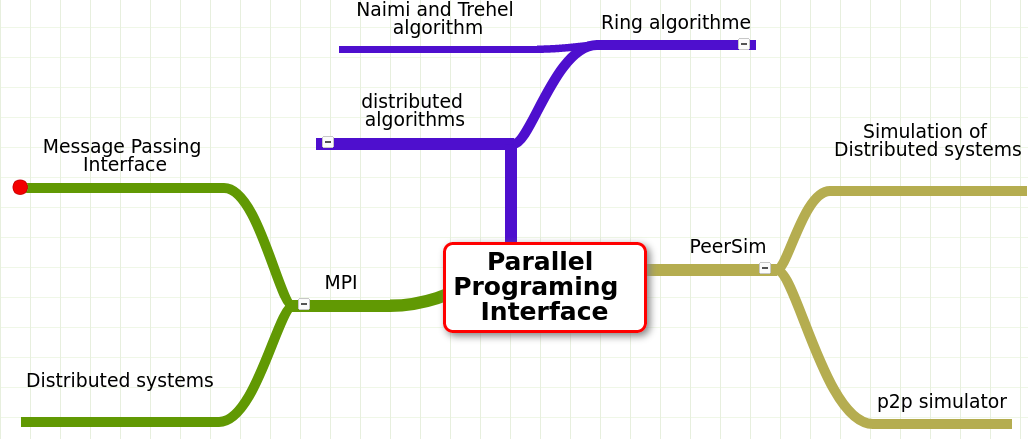
\includegraphics[width=10cm]{mindmap.png}
		\section{Descriptif de la recherche documentaire}
		\indent Nous avons commencé par comprendre ce qu'est un systeme distribué et comment fonctionnent les system MPI et PeerSim a traver quelque exemples d'algorithm que nous avons implémenter dans chaque
		\indent une des API ,nous avons aussi utiliser google scholar pour commprendre comment la communauter utilise les deux API et pour avoir la version exacte et prouver des algorithme que nous avons utiliser
		\indent car pour les algorithme il est facil de passer a côter et beaucoup de gens implémente des version fonctionnel mais qui n'applique pas vraiment l'algorithm c'est pour ça que nous avons utiliser 
		\indent la description de l'algorithme sortie direct des thése des inventeur , pour les deux API nous avons utiliser les manuel des developpeur qui ont créer les deux applications pour mieux comprendre 
		\indent les subtiliter de celle-ci nous avons utiliser la documentation des inventeur car elle est précise et bien détailier.
		\newline
		\indent Nous avons beaucoup utiliser google scholar car il a une quantiter impressionante de ressource et que elle sont pour la plupart des sources fiable et nous a permis d'acceder au thése qui nous
		\indent intéresser, aussi nous avons utiliser la doc du langage Java , vue que ça a était notre langage d'implantation de notre interface.

		
		\section{Bibliographie produite dans le cadre du projet}

		\section{Evaluation des sources}

\end{document}